\documentclass[a4paper]{article}

\usepackage[english]{babel}
\usepackage[utf8]{inputenc}
\usepackage{amsmath}
\usepackage{graphicx}
\usepackage{amsfonts}
%\usepackage{bbm}
\usepackage{tgpagella}
\usepackage[T1]{fontenc}
\usepackage{hyperref}

\title{LDPC codes: Sum Product Algorithm}

\author{Sasank Chilamkurthy, Tharun Kumar Reddy, Varun Bairaboina}

\date{25 April 2014}

\begin{document}
\maketitle

%\begin{abstract}
%We will implement two algorithms each from one of the two important aspects of information theory, which we have background on:
%Source Coding and channel coding.
%\end{abstract}


	\section{Introduction}
    Low Density Parity Check codes are capacity achieving codes proposed with very large parity check matrix. But we
    choose parity check matrix to be sparse, which helps in decoding. In general, decoding of a
    code amounts to finding hamming distance between received binary vector and all codevectors 
    and return the codeword with least distance. Since we are doing block coding, we have 
    $2^n$ codewords to search, where $n$ is length of code-word/vector.
    
    Our method of decoding, though not optimal, uses graph structure of parity check matrix and 
    pass messages/beliefs on the graph. This algorithm is called sum-product algorithm on 
    a factor graph or belief propogation. 
    
    In this report we’ll not give proof why our algorithm works but we’ll give 
    semantics of the algorithm as there are many papers/books dealing with this. Our reference 
    was D McKay, Information Theory, Inference, and Learning Algorithms 
    
    \section{How is decoding done?}
    \textbf{What we have: } A large parity check matrix $H$. Received binary vector $\mathbf{x}$, which is $\mathbb{F}_2$ sum (same as bitwise xor) of a code word $\mathbf{c}$ and a binary noise vector $\mathbf{n}$. i.e. $\mathbf{x}$ = $\mathbf{c}$ + $\mathbf{n}$. All code words satisfy $H\mathbf{x} = 0$.
    \\*
    \\*
    \textbf{What we want to find: }
    Most probable noise vector $\mathbf{\hat{n}}$ that explains received vector  $\mathbf{x}$. Then we can recover original code word by subtracting (same as bitwise xor for $\mathbb{F}_2$) $\mathbf{\hat{n}}$ from $\mathbf{x}$. Define syndrome as $\mathbf{z} = H\mathbf{x}$
    
    $$z =Hx= H(c + n) = Hc + Hn = Hn$$
    \\Thus, our noise estimate $\mathbf{n}$ has to satisfy $\mathbf{z} = H\mathbf{n}$. So, our problem is to find most probable $\mathbf{\hat{n}}$ which satisfy $H\mathbf{\hat{n}} = \mathbf{z}$ where
    \begin{align*}
    P(\mathbf{n},\mathbf{z}) &= P(\mathbf{n}) \mathbf{1}[\mathbf{z} = H\mathbf{n}]\\
    &= \prod_{n}  P(n_n)\prod_{m} \mathbf{1}[z_m = \sum_{n \in \mathcal{N}(m)} n_n]
    \end{align*}
    \\ where  $\mathcal{N}(m)$ denotes set of indices with non-zero elements in $m th$  row. We also introduce notation $\mathcal{M}(n)$ which denotes set of indices with non-zero elements in $n th$  coloumn. 
\\ Since we want to do bit wise decoding, we want to marginalise above function to find $P(n_i=0)$ for each $i$, so as to declare $i th$ bit to be $0$ if this is greater than 0.5 and $1$ otherwise.

\section{Graph Corresponding to a Code}
Parity check matrix H defines a unique bi-partite graph as follows:
\\* Let H be $m  \times n$ matrix. This means code vector is of length n and there are m parity checks. $mth$ parity check checks the parity of bits from set   $\mathcal{N}(m)$. Similarly $nth$ bit occurs in parity check equations indexed by set $\mathcal{M}(n)$. This allows to define a bipartite graph with bits and parity checks as nodes. There is a edge between $nth$ \textit{bit node} and $mth$ \textit{check node} bit $n$ participates in $mth$ parity check equation. This graph is called Tanner Graph.

Let's illustrate this with a (6,3) linear block code with the following parity check matrix:
$$\begin{bmatrix}
1 &1 &1 &0 &1 &0\\
1 &1 &0 &1 &0 &1\\
1 &0 &1 &1 &1 &1\\
\end{bmatrix}$$
Corresponding Tanner Graph is
\\
\begin{center}
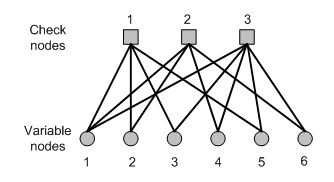
\includegraphics[width=200pt]{image71.jpeg}
\end{center}



\section{Decoding using sum product algorithm}
\textbf{notation: }$\mathbf{r_{mn}}$ is the message passed from check nodes to bit nodes and  $\mathbf{q_{mn}}$ is the message passed from bit nodes to check nodes. These are meant to be beliefs held by check nodes and bit nodes respectively about noise vector $\mathbf{\hat{n}}$ and are vectors of length 2.
\subsection* {Initialization: }
Initialize for every $(n,m)$, $\mathbf{q_{nm}} = [1-f, f] $ where f is probability of error. This is initial belief held by bit nodes about  $n th$ bit of noise vector.

\subsection*{Horizontal step: }
In Horizontal step (horizontal from the point of view of $H$), we compute $\mathbf{r_{mn}}$ which is belief held by $m th$ check node about $n th$ bit node. It is calculated by considering beliefs of all bit nodes received by  $m th$ check node except $n th$ bit node.
\begin{align*}
\mathbf{r_{mn}}[0]  &= \sum_{{x_n' : n' \in \mathcal{N}(m)\backslash n }} \mathbf{1}[z_m  =  \sum x_n'] \prod_{ n' \in \mathcal{N}(m)\backslash n} q_{mn'} [x_{n'}]  \\
\mathbf{r_{mn}}[1]  &=  1 - \mathbf{r_{mn}}[0]
\end{align*}
\subsection*{Vertical step: }
In this step, we compute  $\mathbf{q_{mn}}$ which is the belief held by $nth$ bit node about itself that will be transmitted to  $mth$ check node, considering its own belief and received beliefs from all check nodes except $mth$ check node.

\begin{align*}
\mathbf{q}_{mn}[0]  &=  \alpha *(1-f) \prod_{m' \in \mathcal{M}(n)\backslash m} r_{m'n}[0] \\
\mathbf{q}_{mn}[1]  &=  \alpha *f \prod_{m' \in \mathcal{M}(n)\backslash m} r_{m'n}[1]
\end{align*}
$\alpha$ is chosen such that $\mathbf{q}_{mn}[0] +  \mathbf{q}_{mn}[1]  = 1$
\\In this step we also calculate net belief of $nth$ node about itself. This is computed as 
\begin{align*}
\mathbf{q}_{n}[0]  &=  \beta *(1-f) \prod_{m \in \mathcal{M}(n)} r_{mn}[0] \\
\mathbf{q}_{n}[1]  &=  \beta *f \prod_{m \in \mathcal{M}(n)} r_{mn}[1]
\end{align*}
$\beta$ is chosen such that $\mathbf{q}_{n}[0] +  \mathbf{q}_{n}[1]  = 1$
\\We use these for estimating $\mathbf{\hat{n}}$ as follows:
$\mathbf{\hat{n}}_n = 0 $if $    \mathbf{q}_{n}[0] > 0.5$ and  $= 1$ otherwise
\\*

We now check if this estimate satisfies $H\mathbf{\hat{n}} = \mathbf{z}$. If it does, we have the required estimate and we stop here. If it is not satisfied, we go to Horizontal step. If iteration doesn't stop after fixed number of steps, we stop anyway. Once we have estimate of noise vector $\mathbf{\hat{n}}$, we return decoded codeword $c = \mathbf{x}+ \mathbf{\hat{n}}$

It should be clear why this algorithm is also called Belief Propogation.

\section{Implementation Details}
We created and stored Tanner Graph as adjacency lists storing indices of nodes adjacent to a given node. We used two \texttt{arrayList<arrayList>} for this - one for check nodes and other for bit nodes. We stored messages to be passed in a data structure which we call as \texttt{Table}. It is basically Hashmap with tuples as keys. We implemented this using \texttt{hashMap<hashMap>}.

\section{Analysis}
Parity check matrices for LDPC codes are very sparse. Column and row weights are very small and are in the range of 2 - 10. Thus Horizontal step takes only linear time with $n$, where $n$ is length of code vector. Vertical step also takes linear time. We can compute syndrome/matrix multiplication very efficiently using constructed graph structure in linear time. 
If parity check matrix was not sparse as we assumed, horizontal step takes exponential time!
Summarily, complexity of decoding using sum product algorithm for LDPC codes is $O(n)$

\section{References and Acknowlegements}
Algorithms for lzw encoding and decoding are from Prof.B.K.Dey's slides on source coding. We've learnt sum product algorithm and LDPC codes from D McKay Information Theory, Inference, and Learning Algorithms which is available for free online viewing here: \texttt{\href{http://www.inference.phy.cam.ac.uk/itprnn/book.pdf}{link}}. Complete Bibliography is available in this book.
\\Thanks to Prof.B.K.Dey for suggesting implemetation of sum-product algorithm.
\end{document}